% Chapter Template

\chapter{EDA and classifier performance} % Main chapter title

\label{chapter3} % Change X to a consecutive number; for referencing this chapter elsewhere, use \ref{ChapterX}

\section{EDA}
There are a total of 18829 annotated sentences. Table~\ref{tab:top_10_sentence} and~\ref{tab:bottom_10_sentence} show some summary statistics of the top 10 and bottom 10 frequently occurring practices at the sentence level. 

\begin{table}[!ht]
	\resizebox{\textwidth}{!}{
	\begin{tabular}{lrrrr}
	\toprule
									  practice &  counts &  sentence\_length\_mean &  sentence\_length\_median &  counts\_percentage \\
	\midrule
	Identifier\_Cookie\_or\_similar\_Tech\_1stParty &    2107 &             25.4 &                    22.0 &           11.2\% \\
			   Contact\_E\_Mail\_Address\_1stParty &    2106 &             28.7 &                    25.0 &           11.2\% \\
							 Location\_1stParty &    1514 &             29.2 &                    24.0 &           8.1\% \\
	Identifier\_Cookie\_or\_similar\_Tech\_3rdParty &    1250 &             27.3 &                    24.0 &           6.6\% \\
				Identifier\_IP\_Address\_1stParty &    1005 &             30.9 &                    27.0 &           5.3\% \\
				 Contact\_Phone\_Number\_1stParty &     970 &             29.1 &                    25.0 &           5.2\% \\
				 Identifier\_Device\_ID\_1stParty &     697 &             32.4 &                    28.0 &           3.7\% \\
			   Contact\_Postal\_Address\_1stParty &     597 &             28.9 &                    26.0 &           3.2\% \\
										   SSO &     504 &             32.6 &                    28.0 &           2.7\% \\
					  Demographic\_Age\_1stParty &     428 &             33.1 &                    26.0 &           2.3\% \\
	\bottomrule
	\end{tabular}
	}
	\caption{Summary statistics for top 10 occurring practices at sentence level.}
	\label{tab:top_10_sentence}
	\end{table}

	\begin{table}[!ht]
		\resizebox{\textwidth}{!}{
		\begin{tabular}{lrrrr}
		\toprule
								practice &  counts &  sentence\_length\_mean &  sentence\_length\_median &  counts\_percentage \\
		\midrule
		Identifier\_Mobile\_Carrier\_3rdParty &      35 &             47.1 &                    30.0 &           0.19\% \\
					Contact\_ZIP\_3rdParty &      34 &             40.2 &                    41.0 &           0.18\% \\
		Identifier\_SSID\_BSSID\_1stParty &      33 &             28.1 &                    24.0 &           0.18\% \\
			  Contact\_Password\_3rdParty &      33 &             24.2 &                    20.0 &           0.18\% \\
					Contact\_City\_3rdParty &      24 &             180 &                    14.0 &           0.13\% \\
		Contact\_Address\_Book\_3rdParty &      17 &             39.6 &                    34.0 &           0.1\% \\
			  Identifier\_IMSI\_1stParty &      13 &             48.2 &                    44.0 &           0.07\% \\
		Identifier\_SIM\_Serial\_3rdParty &       5 &             41.2 &                    54.0 &           0.03\% \\
			  Identifier\_IMSI\_3rdParty &       4 &             54.3 &                    47.5 &           0.02\% \\
		Identifier\_SSID\_BSSID\_3rdParty &       2 &             65.5 &                    65.5 &           0.01\% \\
		\bottomrule
	\end{tabular}
	}
	\caption{Summary statistics for bottom 10 frequently occurring practices.}
	\label{tab:bottom_10_sentence}
\end{table}

In total, the top 10 frequently occurring practices make up approximately 60\% of the dataset. The bottom 10 frequently occurring practices make up approximately 1\% of the dataset.

According to Table~\ref{tab:summary_top_10_practices}, there does not seem to be much variation in sentence length for the top 10 frequently occurring practices, since the standard deviation for the mean is approximately 2.5 words and the median 1.9 words. This could indicate similar sentence complexity across the practices.

\begin{table}[!ht]
	\centering
	\begin{tabular}{lrr}
		\toprule
		{} &  sentence\_length\_mean &  sentence\_length\_median \\
		\midrule
		count &             10.000000 &               10.000000 \\
		mean  &             29.747511 &               25.500000 \\
		std   &              2.468191 &                1.900292 \\
		min   &             25.389654 &               22.000000 \\
		25\%   &             28.715572 &               24.250000 \\
		50\%   &             29.138353 &               25.500000 \\
		75\%   &             32.011357 &               26.750000 \\
		max   &             33.074766 &               28.000000 \\
		\bottomrule
	\end{tabular}
	\caption{Summary sentence statistics for top 10 frequently occurring practices.}
	\label{tab:summary_top_10_practices}
\end{table}

\begin{figure}[!ht]
	\begin{subfigure}[b]{1\linewidth}
	  \centering
	  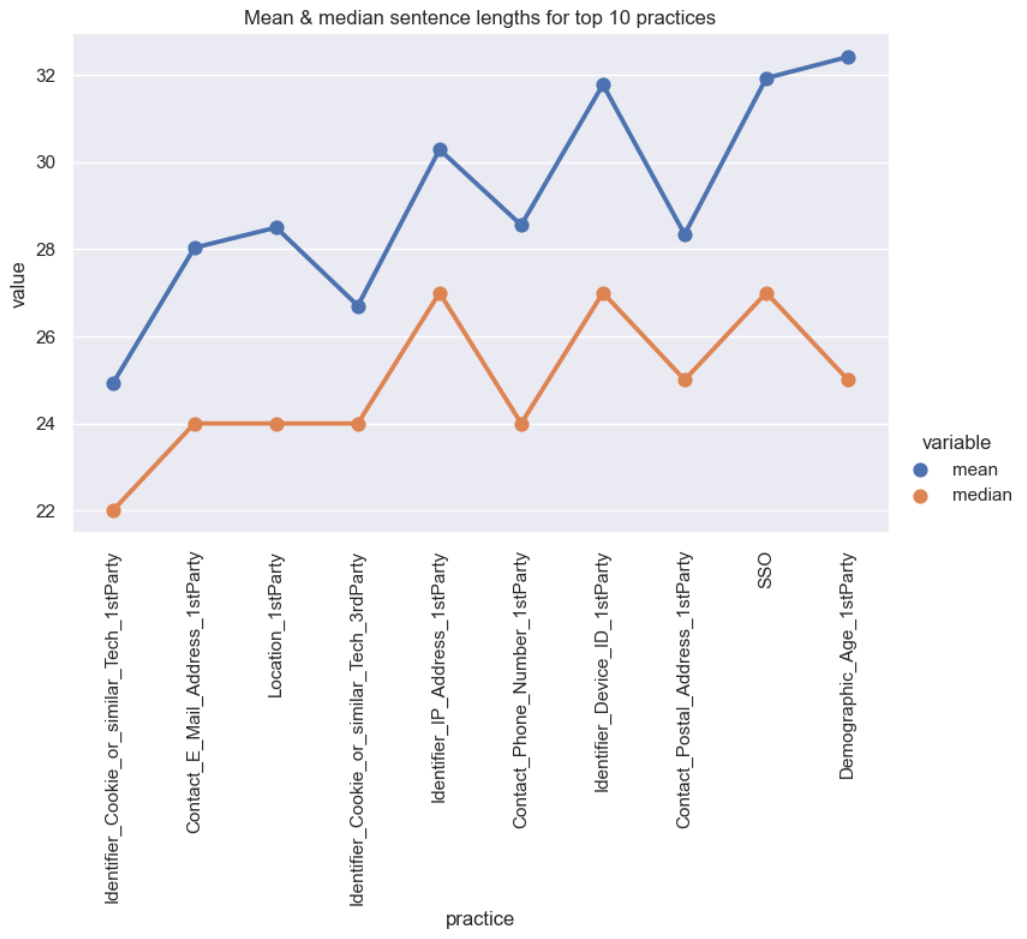
\includegraphics[width=0.85\linewidth]{figures/eda_mean_median.png}
	  \caption{Mean and median sentence length}
	\end{subfigure}
	\hfill
	\begin{subfigure}[b]{1\linewidth}
	  \centering
	  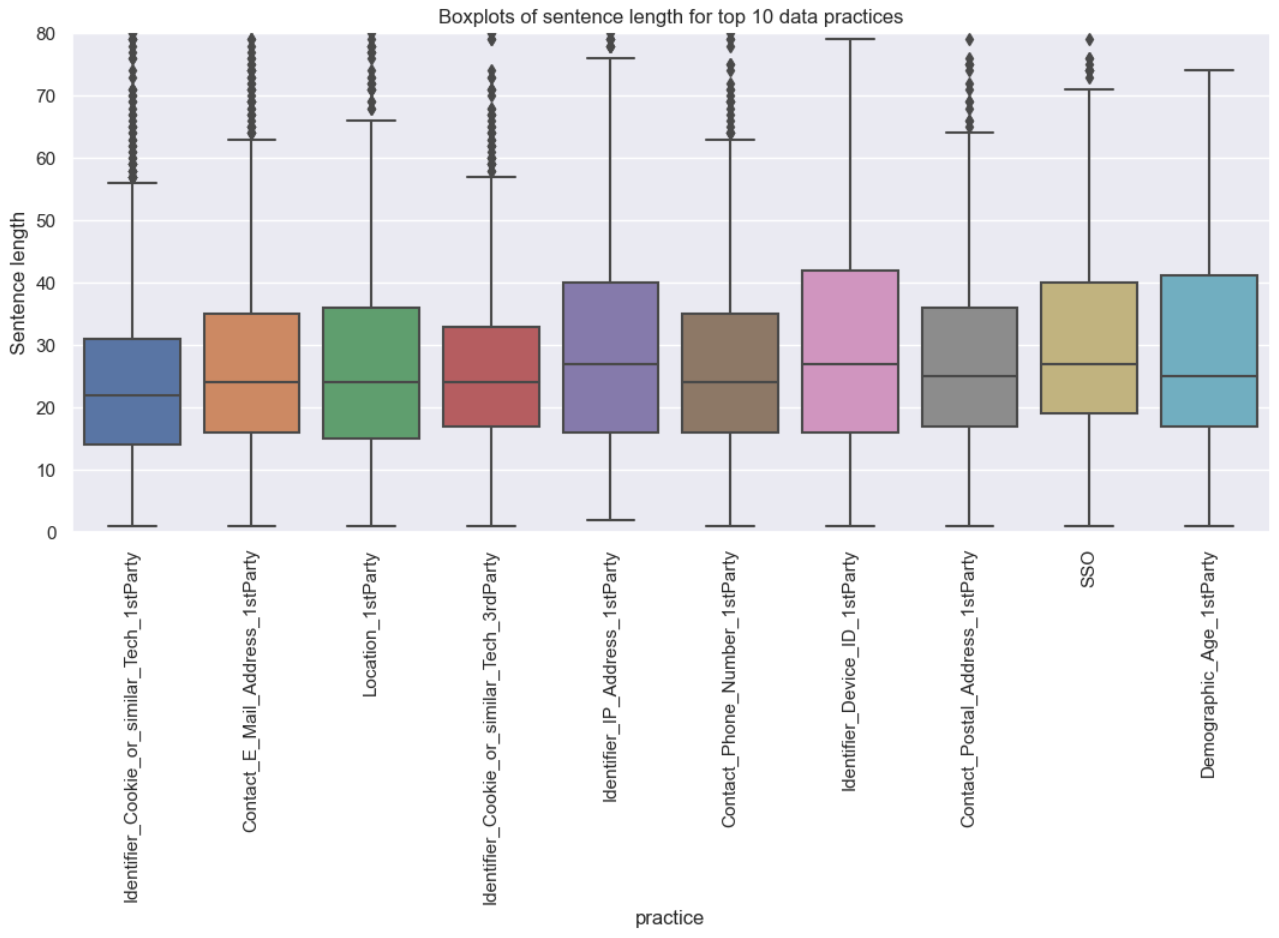
\includegraphics[width=0.85\linewidth]{figures/eda_boxplots.png}
	  \caption{Boxplots of sentence length (note: not all outliers shown to focus on visualising IQR)}
	\end{subfigure}
	\caption{Summary plots for top 10 frequently occurring data practices (Practices shown in order of descending frequency)}
	\label{fig:eda}
\end{figure}


\begin{figure}[!ht]
	\begin{subfigure}[t]{.5\textwidth}
	  \centering
	  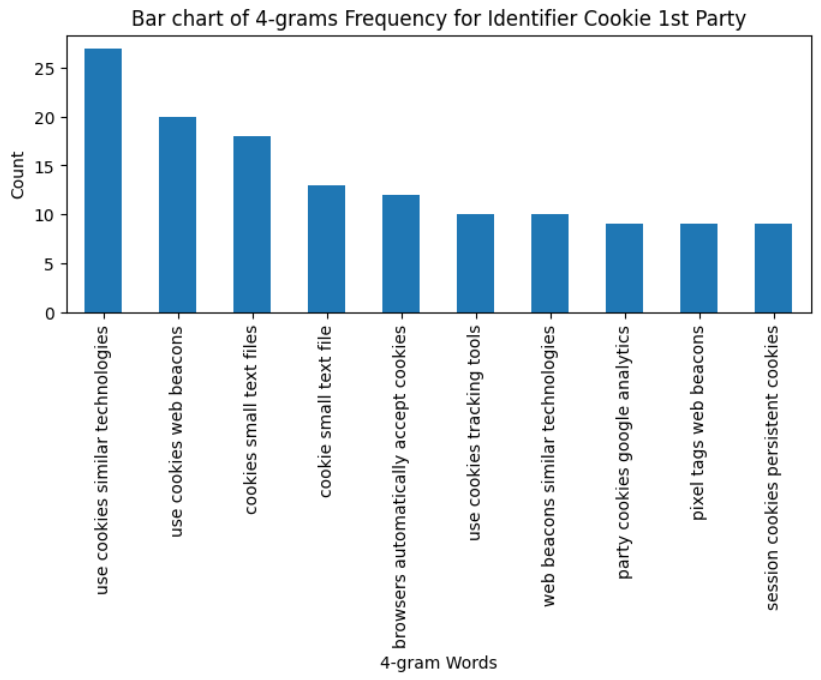
\includegraphics[width=\linewidth]{figures/4_grams_cookie_1stParty.png}
	  \caption{Identifier Cookie 1st Party}
	\end{subfigure}
	\hfill
	\begin{subfigure}[t]{.5\textwidth}
	  \centering
	  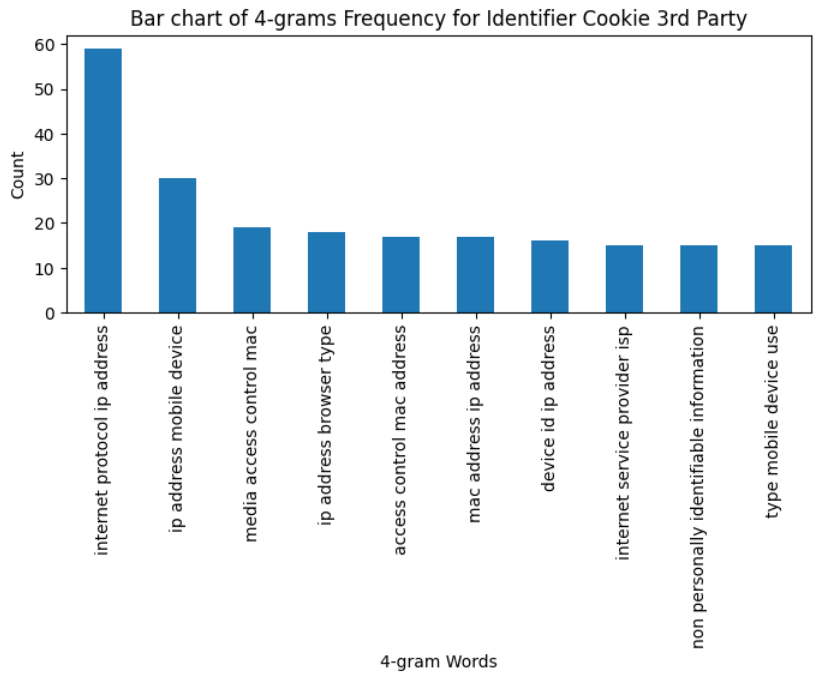
\includegraphics[width=\linewidth]{figures/4_grams_cookie_3rdParty.png}
	  \caption{Identifier Cookie 3rd Party}
	\end{subfigure}
	
	\medskip
  
	\begin{subfigure}[t]{.5\textwidth}
	  \centering
	  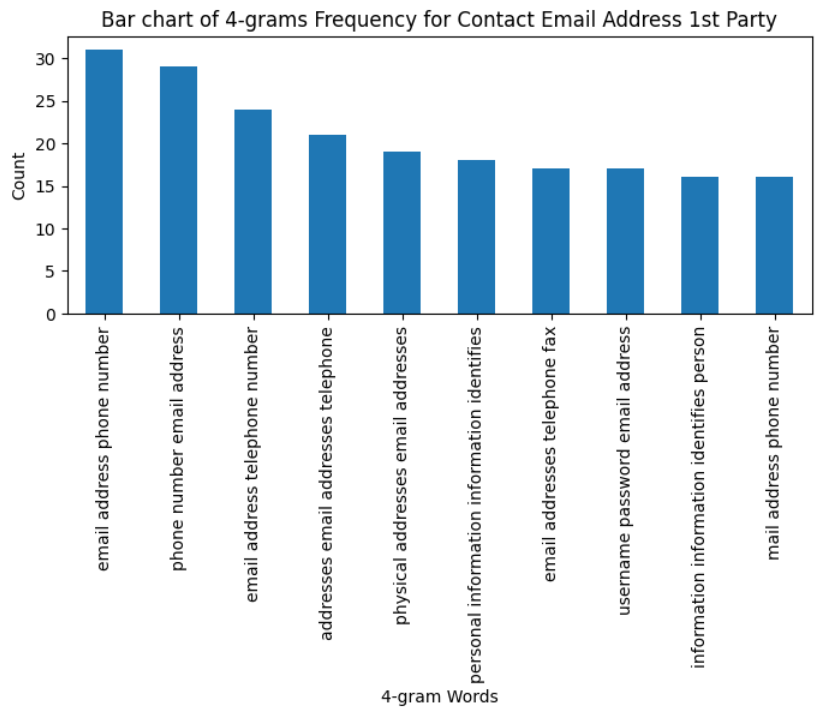
\includegraphics[width=\linewidth]{figures/4_grams_email.png}
	  \caption{Identifier Email}
	\end{subfigure}
	\hfill
	\begin{subfigure}[t]{.5\textwidth}
	  \centering
	  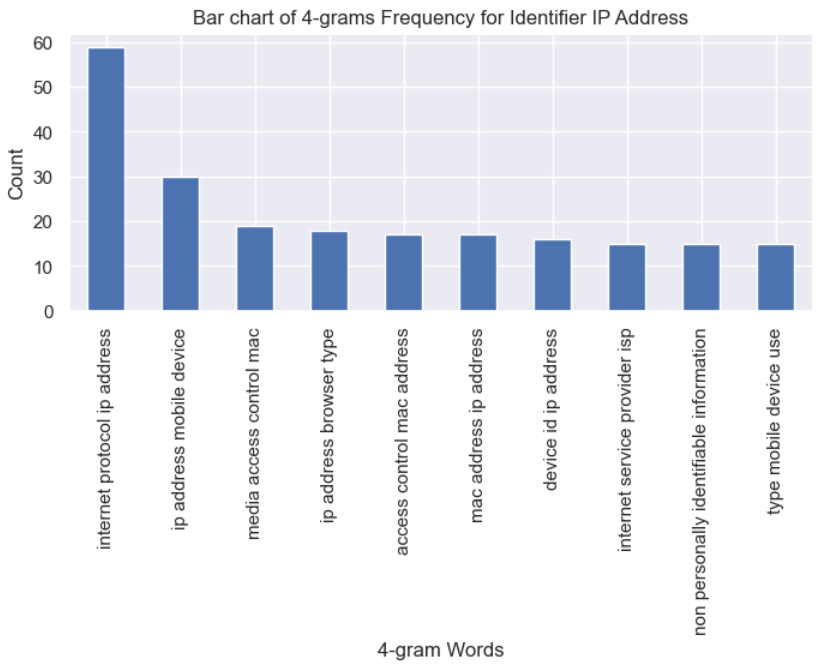
\includegraphics[width=\linewidth]{figures/4_grams_ip_address.png}
	  \caption{Identifier IP Address}
	\end{subfigure}
	\begin{subfigure}[t]{.5\textwidth}
		\centering
		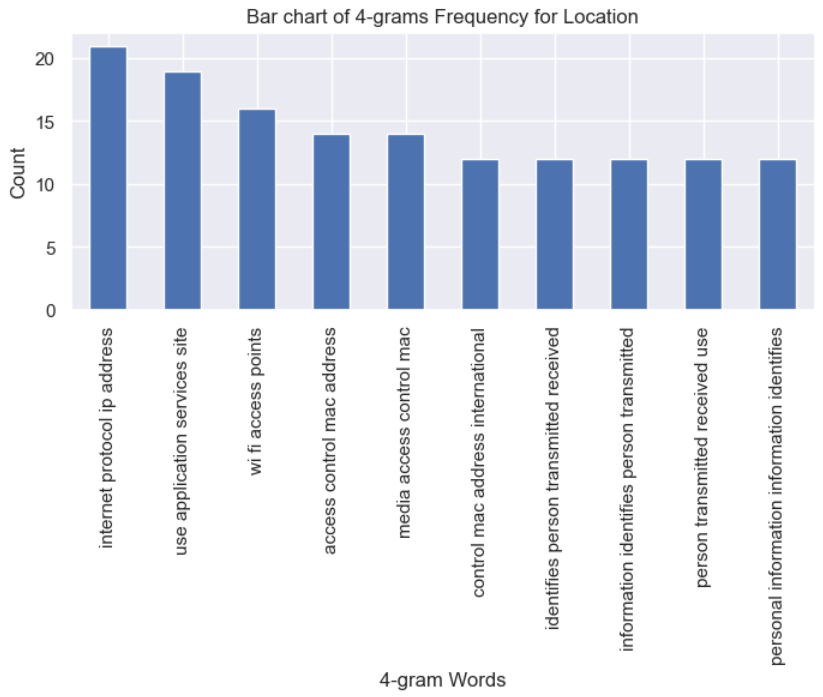
\includegraphics[width=\linewidth]{figures/4_grams_location.png}
		\caption{Location 1st Party}
	\end{subfigure}
	\caption{Top 10 most frequently occurring 4-grams in the top most frequently occurring 5 data practices at the sentence level}
	\label{fig:4_grams_sentence}
  \end{figure}


\section{Models used and classification metrics}
I use Logistic Regression, SGDClassifier and SVC classifiers and compare the weighted precision, recall and F1 scores. Precision, Recall and F1 scores different metrics are used to assess the performance of classifiers. They are stated mathematically below.
\begin{align*}
	\text{Precision} &= \frac{\text{True Positive}}{\text{True Positive + False Positive}} \\
	\text{Recall} &= \frac{\text{True Positive}}{\text{True Positive + False Negative}} \\
	\text{F1} &= 2 \cdot \frac{\text{Precision} \cdot \text{Recall}}{\text{Precision + Recall}}
\end{align*}
Since there is neither a high risk of identifying false positives or false negatives, F1 score is primarily used to assess the performance for the models. As the distributions of records across the practices are uneven, I focus on the weighted average of F1 scores as the most important indicator of model performance. 

\section{Performance of classifiers for top N practices}
As seen in Table~\ref{tab:top_10_sentence} above, there is an uneven distribution of records across the practices. Further, the bottom 10 frequently occurring practices only contains about 2 to 35 records for each practice. Given that there are in total 57 practices for the entire dataset, and there is not a uniform distribution of occurrences. Training models on all 57 practices would likely lead to low performance since there are not enough records for all 57 practices. Thus, to find an optimal balance between model performance and still maintain a realistic sample of practices that could appear in a real world dataset, I chose to assess model performance by first assessing the performance of the three classifiers paired with Tf-IDF for the top N (where $3 \le N \le 10$) frequently occurring practices. The metrics are in Figure~\ref{fig:top_n_practices}.

Generally we see that the SVC classifier performs the best across the metrics and across the top N frequently occurring practices for both sentence and segment level. This corresponds with the findings by the researchers as they also found that the SVC classifier produced the best performance. Also, performance of all the models generally decreases with increasing $N$, which is not surprising since it gets harder for the classifier to find a decision boundary with more classes.

\begin{figure}[!ht]
	\centering
	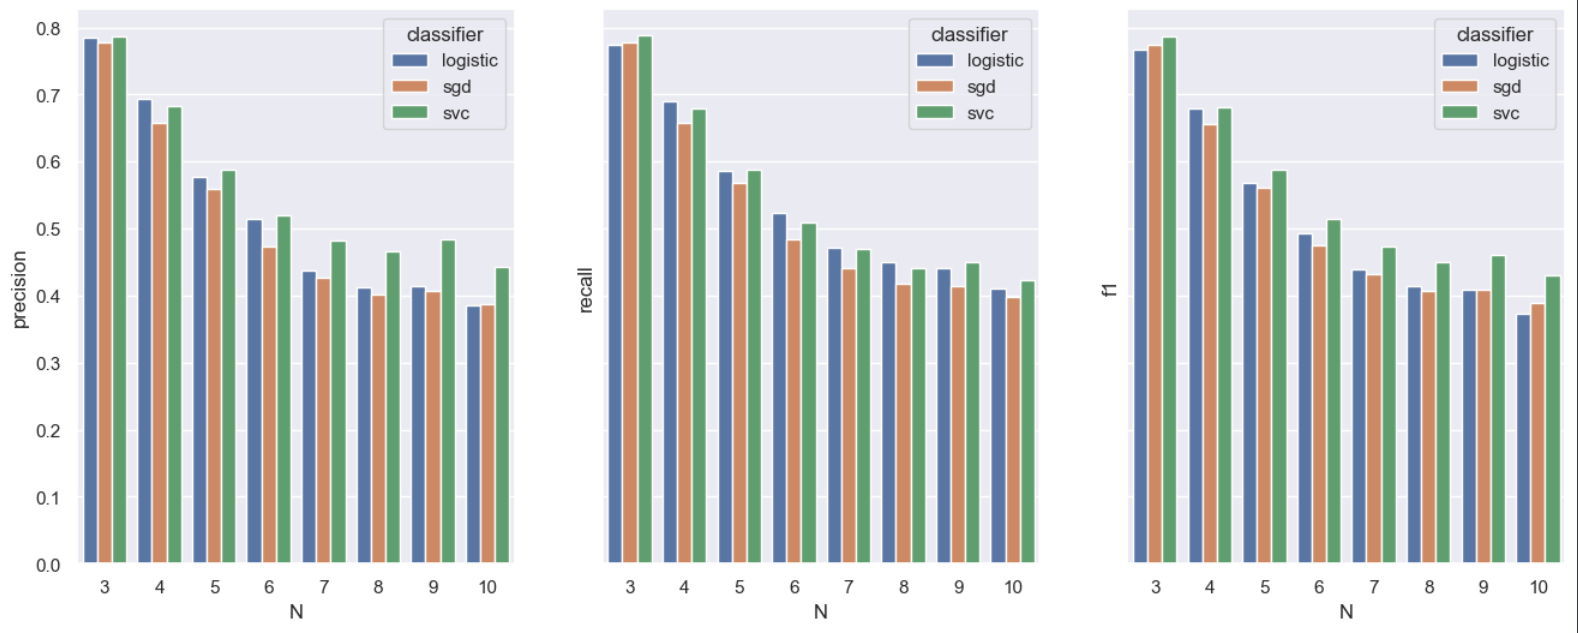
\includegraphics[width=1\textwidth]{figures/model_n_testing_sentence.png}      
    \caption{Weighted average P/R/F1 scores for top N ($3 \le N \le 10$) practices}
    \label{fig:top_n_practices}
\end{figure}


%----------------------------------------------------------------------------------------
%	SECTION 2
%----------------------------------------------------------------------------------------

\section{Performance of individual classifiers for top 5 practices}
Since SGDClassifier performed similarly to the 2 other classifiers, I focus only on comparing logistic regression and SVC, with logistic regression as the baseline classifier and SVC since the APP-350 researchers used SVC. I also compare the performance of Tf-IDF and GloVe. In total, I documented the performance of all 4 possible combinations of text representations and models in Figures~\ref{fig:heatmaps_perf_lr} and~\ref{fig:heatmaps_perf_svc} show the averaged metrics over a 5-fold cross validation. 

Similarly to what Zimmeck et al. found, SVC + Tf-IDF provided the best overall performance with the weighted average at 66\%. This is quite a significant performance difference from the lowest performing model, logistic regression + GloVe at 54\%. Specifically for \texttt{Identifier Cookie 1st Party}, both logistic regression + Tf-IDF and SVC + Tf-IDF performed similarly at 68\% F1, but SVC + Tf-IDF had a more balanced performance across precision and recall. Overall, these performance figures confirm that SVC is the better performing model, though the performance difference between the benchmark logistic regression model and SVC is not that significant (from 62\% to 66\% weighted average F1). It is also interesting to note that GloVe embeddings performed worse compared to Tf-IDF regardless of the model used, when GloVe is the more sophisticated text representation given that only GloVe vectors capture the context of the word. Further, these results seem to correspond with a study measuring performance of supervised machine learning for classification tasks using generalised text datasets (\cite{hsu2020}). LinearSVC followed by logistic regression were the highest performing models, with AdaBoost and Decision Trees having comparatively lower performance.

\begin{figure}[!ht]
	\begin{subfigure}[b]{1\textwidth}
	  \centering
	  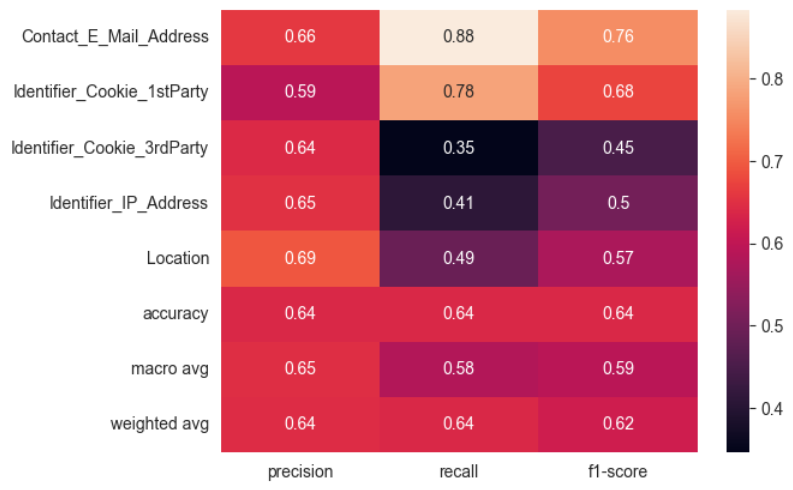
\includegraphics[width=\linewidth]{figures/heatmap_log_tfidf.png}
	  \caption{Logistic regression + TfIDF}
	\end{subfigure}
	\hfill
	\begin{subfigure}[b]{1\textwidth}
	  \centering
	  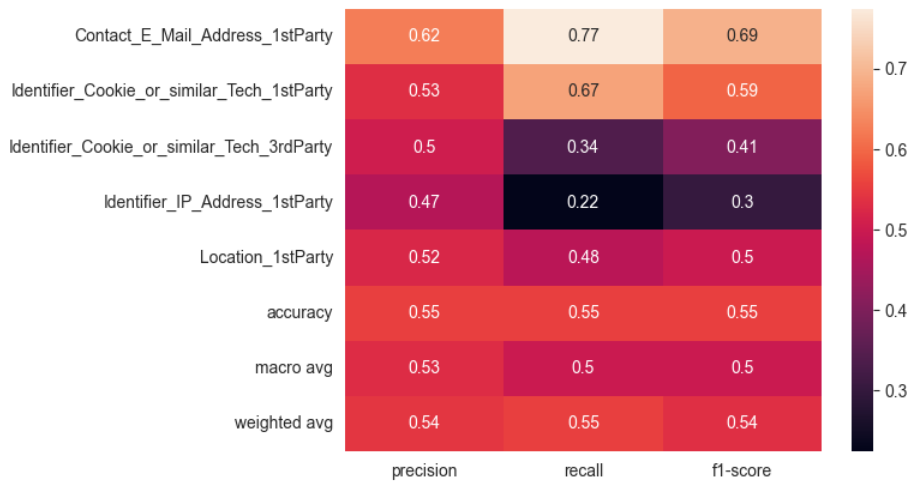
\includegraphics[width=\linewidth]{figures/heatmap_log_glove.png}
	  \caption{Logistic regression + GloVe}
	\end{subfigure}
	\caption{Performance heatmaps of logistic regression classifiers}
	\label{fig:heatmaps_perf_lr}
\end{figure}
	
\begin{figure}[!ht]
	\begin{subfigure}[b]{1\textwidth}
	  \centering
	  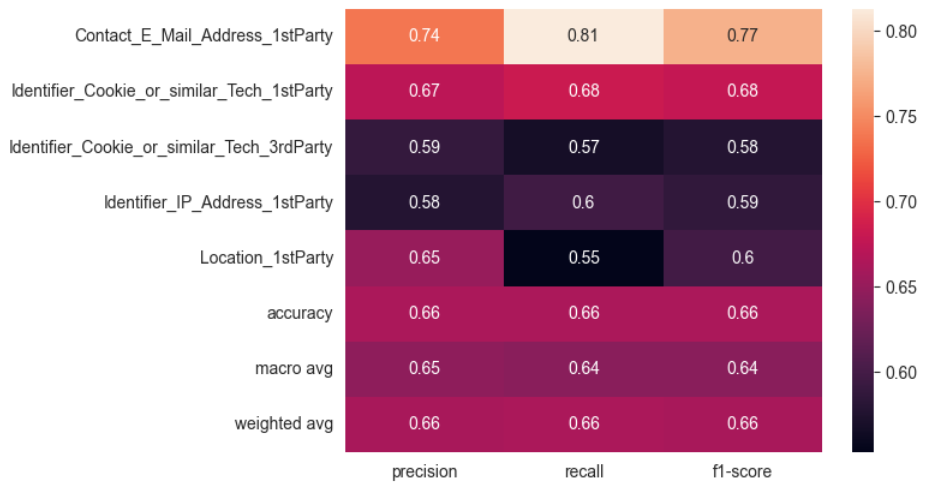
\includegraphics[width=\linewidth]{figures/heatmap_svc_tfidf.png}
	  \caption{SVC + TfIDF}
	\end{subfigure}
	\hfill
	\begin{subfigure}[b]{1\textwidth}
	  \centering
	  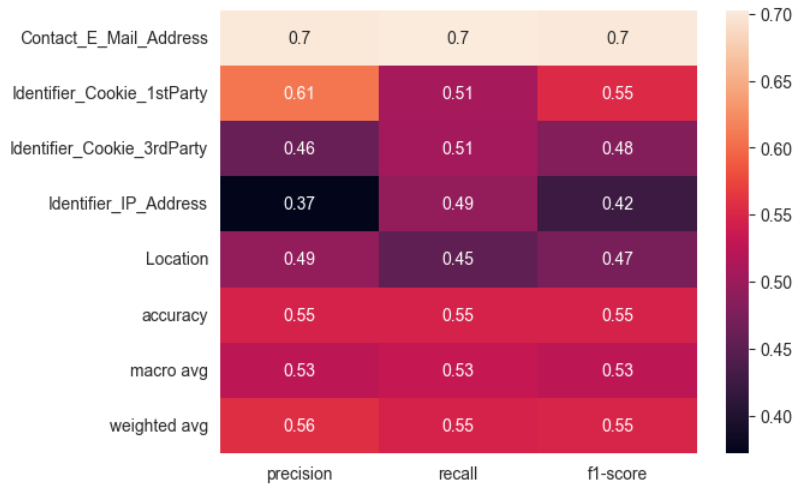
\includegraphics[width=\linewidth]{figures/heatmap_svc_glove.png}
	  \caption{SVC + GloVe}
	\end{subfigure}
	\caption{Performance heatmaps of SVC classifiers}
	\label{fig:heatmaps_perf_svc}
\end{figure}

% \begin{table}[!ht]
% 	\resizebox{\textwidth}{!}{
% 		\begin{tabular}{lllll}
% 		\hline
% 		\multicolumn{1}{|l|}{\textbf{Data Practice}}          & \multicolumn{1}{l|}{\textbf{Precision}} & \multicolumn{1}{l|}{\textbf{Recall}} & \multicolumn{1}{l|}{\textbf{F1}} & \multicolumn{1}{l|}{\textbf{Support}} \\ \hline
% 		\multicolumn{1}{|l|}{Contact Email Address 1st Party} & \multicolumn{1}{l|}{0.66}               & \multicolumn{1}{l|}{0.88}            & \multicolumn{1}{l|}{0.76}        & \multicolumn{1}{l|}{2106}              \\ \hline
% 		\multicolumn{1}{|l|}{Identifier Cookie 1st Party}    & \multicolumn{1}{l|}{0.59}               & \multicolumn{1}{l|}{0.78}            & \multicolumn{1}{l|}{0.68}        & \multicolumn{1}{l|}{2107}              \\ \hline
% 		\multicolumn{1}{|l|}{Identifier Cookie 3rd Party}     & \multicolumn{1}{l|}{0.64}               & \multicolumn{1}{l|}{0.35}            & \multicolumn{1}{l|}{0.45}        & \multicolumn{1}{l|}{1250}              \\ \hline
% 		\multicolumn{1}{|l|}{Identifier IP Address 1st Party} & \multicolumn{1}{l|}{0.66}               & \multicolumn{1}{l|}{0.41}            & \multicolumn{1}{l|}{0.50}        & \multicolumn{1}{l|}{1005}              \\ \hline
% 		\multicolumn{1}{|l|}{Location 1st Party}              & \multicolumn{1}{l|}{0.69}               & \multicolumn{1}{l|}{0.49}            & \multicolumn{1}{l|}{0.57}        & \multicolumn{1}{l|}{1514}              \\ \hline
% 																&                                         &                                      &                                  &                                       \\ \hline
% 		\multicolumn{1}{|l|}{\textbf{accuracy}}               & \multicolumn{1}{l|}{}                   & \multicolumn{1}{l|}{}                & \multicolumn{1}{l|}{0.64}        & \multicolumn{1}{l|}{7982}             \\ \hline
% 		\multicolumn{1}{|l|}{\textbf{macro avg}}              & \multicolumn{1}{l|}{0.65}               & \multicolumn{1}{l|}{0.58}            & \multicolumn{1}{l|}{0.59}        & \multicolumn{1}{l|}{7982}             \\ \hline
% 		\multicolumn{1}{|l|}{\textbf{weighted avg}}           & \multicolumn{1}{l|}{0.64}               & \multicolumn{1}{l|}{0.64}            & \multicolumn{1}{l|}{0.62}        & \multicolumn{1}{l|}{7982}             \\ \hline
% 		\end{tabular}
% 	}
% 	\caption{Logistic regression + Tf-IDF}
% 	\label{tab:lr+tfidf}
% \end{table}


% \begin{table}[!ht]
% 	\resizebox{\textwidth}{!}{
% 		\begin{tabular}{lllll}
% 		\hline
% 		\multicolumn{1}{|l|}{\textbf{Data Practice}}          & \multicolumn{1}{l|}{\textbf{Precision}} & \multicolumn{1}{l|}{\textbf{Recall}} & \multicolumn{1}{l|}{\textbf{F1}} & \multicolumn{1}{l|}{\textbf{Support}} \\ \hline
% 		\multicolumn{1}{|l|}{Contact Email Address 1st Party} & \multicolumn{1}{l|}{0.62}               & \multicolumn{1}{l|}{0.77}            & \multicolumn{1}{l|}{0.70}        & \multicolumn{1}{l|}{2106}              \\ \hline
% 		\multicolumn{1}{|l|}{Identifier Cookie 1st Party}    & \multicolumn{1}{l|}{0.53}               & \multicolumn{1}{l|}{0.67}            & \multicolumn{1}{l|}{0.59}        & \multicolumn{1}{l|}{2107}              \\ \hline
% 		\multicolumn{1}{|l|}{Identifier Cookie 3rd Party}     & \multicolumn{1}{l|}{0.50}               & \multicolumn{1}{l|}{0.34}            & \multicolumn{1}{l|}{0.41}        & \multicolumn{1}{l|}{1250}              \\ \hline
% 		\multicolumn{1}{|l|}{Identifier IP Address 1st Party} & \multicolumn{1}{l|}{0.47}               & \multicolumn{1}{l|}{0.22}            & \multicolumn{1}{l|}{0.30}        & \multicolumn{1}{l|}{1005}              \\ \hline
% 		\multicolumn{1}{|l|}{Location 1st Party}              & \multicolumn{1}{l|}{0.52}               & \multicolumn{1}{l|}{0.48}            & \multicolumn{1}{l|}{0.50}        & \multicolumn{1}{l|}{1514}              \\ \hline
% 																&                                         &                                      &                                  &                                       \\ \hline
% 		\multicolumn{1}{|l|}{\textbf{accuracy}}               & \multicolumn{1}{l|}{}                   & \multicolumn{1}{l|}{}                & \multicolumn{1}{l|}{0.55}        & \multicolumn{1}{l|}{7982}             \\ \hline
% 		\multicolumn{1}{|l|}{\textbf{macro avg}}              & \multicolumn{1}{l|}{0.53}               & \multicolumn{1}{l|}{0.50}            & \multicolumn{1}{l|}{0.50}        & \multicolumn{1}{l|}{7982}             \\ \hline
% 		\multicolumn{1}{|l|}{\textbf{weighted avg}}           & \multicolumn{1}{l|}{0.54}               & \multicolumn{1}{l|}{0.55}            & \multicolumn{1}{l|}{0.54}        & \multicolumn{1}{l|}{7982}             \\ \hline
% 		\end{tabular}
% 	}
% 	\caption{Logistic regression + GloVe embeddings}
% 	\label{tab:lr+glove}
% \end{table}


% \begin{table}[!ht]
% 	\resizebox{\textwidth}{!}{
% 	\begin{tabular}{lllll}
% 		\hline
% 		\multicolumn{1}{|l|}{\textbf{Data Practice}}          & \multicolumn{1}{l|}{\textbf{Precision}} & \multicolumn{1}{l|}{\textbf{Recall}} & \multicolumn{1}{l|}{\textbf{F1}} & \multicolumn{1}{l|}{\textbf{Support}} \\ \hline
% 		\multicolumn{1}{|l|}{Contact Email Address 1st Party} & \multicolumn{1}{l|}{0.74}               & \multicolumn{1}{l|}{0.81}            & \multicolumn{1}{l|}{0.77}        & \multicolumn{1}{l|}{2106}              \\ \hline
% 		\multicolumn{1}{|l|}{Identifier Cookie 1st Party}     & \multicolumn{1}{l|}{0.67}               & \multicolumn{1}{l|}{0.68}            & \multicolumn{1}{l|}{0.68}        & \multicolumn{1}{l|}{2107}              \\ \hline
% 		\multicolumn{1}{|l|}{Identifier Cookie 3rd Party}     & \multicolumn{1}{l|}{0.59}               & \multicolumn{1}{l|}{0.57}            & \multicolumn{1}{l|}{0.58}        & \multicolumn{1}{l|}{1250}              \\ \hline
% 		\multicolumn{1}{|l|}{Identifier IP Address 1st Party} & \multicolumn{1}{l|}{0.58}               & \multicolumn{1}{l|}{0.60}            & \multicolumn{1}{l|}{0.59}        & \multicolumn{1}{l|}{1005}              \\ \hline
% 		\multicolumn{1}{|l|}{Location 1st Party}              & \multicolumn{1}{l|}{0.65}               & \multicolumn{1}{l|}{0.55}            & \multicolumn{1}{l|}{0.60}        & \multicolumn{1}{l|}{1514}              \\ \hline
% 																&                                         &                                      &                                  &                                       \\ \hline
% 		\multicolumn{1}{|l|}{\textbf{accuracy}}               & \multicolumn{1}{l|}{}                   & \multicolumn{1}{l|}{}                & \multicolumn{1}{l|}{0.66}        & \multicolumn{1}{l|}{7982}             \\ \hline
% 		\multicolumn{1}{|l|}{\textbf{macro avg}}              & \multicolumn{1}{l|}{0.65}               & \multicolumn{1}{l|}{0.64}            & \multicolumn{1}{l|}{0.64}        & \multicolumn{1}{l|}{7982}             \\ \hline
% 		\multicolumn{1}{|l|}{\textbf{weighted avg}}           & \multicolumn{1}{l|}{0.66}               & \multicolumn{1}{l|}{0.66}            & \multicolumn{1}{l|}{0.66}        & \multicolumn{1}{l|}{7982}             \\ \hline
% 		\end{tabular}
% 	}
% 	\caption{SVC + Tf-IDF}
% 	\label{tab:svc+tfidf}
% \end{table}

% \begin{table}[!ht]
% 	\resizebox{\textwidth}{!}{
% 	\begin{tabular}{lllll}
% 		\hline
% 		\multicolumn{1}{|l|}{\textbf{Data Practice}}          & \multicolumn{1}{l|}{\textbf{Precision}} & \multicolumn{1}{l|}{\textbf{Recall}} & \multicolumn{1}{l|}{\textbf{F1}} & \multicolumn{1}{l|}{\textbf{Support}} \\ \hline
% 		\multicolumn{1}{|l|}{Contact Email Address 1st Party} & \multicolumn{1}{l|}{0.70}               & \multicolumn{1}{l|}{0.70}            & \multicolumn{1}{l|}{0.70}        & \multicolumn{1}{l|}{2106}              \\ \hline
% 		\multicolumn{1}{|l|}{Identifier Cookie 1st Party}     & \multicolumn{1}{l|}{0.61}               & \multicolumn{1}{l|}{0.51}            & \multicolumn{1}{l|}{0.55}        & \multicolumn{1}{l|}{2107}              \\ \hline
% 		\multicolumn{1}{|l|}{Identifier Cookie 3rd Party}     & \multicolumn{1}{l|}{0.46}               & \multicolumn{1}{l|}{0.51}            & \multicolumn{1}{l|}{0.48}        & \multicolumn{1}{l|}{1250}              \\ \hline
% 		\multicolumn{1}{|l|}{Identifier IP Address 1st Party} & \multicolumn{1}{l|}{0.37}               & \multicolumn{1}{l|}{0.49}            & \multicolumn{1}{l|}{0.42}        & \multicolumn{1}{l|}{1005}              \\ \hline
% 		\multicolumn{1}{|l|}{Location 1st Party}              & \multicolumn{1}{l|}{0.49}               & \multicolumn{1}{l|}{0.45}            & \multicolumn{1}{l|}{0.47}        & \multicolumn{1}{l|}{1514}              \\ \hline
% 																&                                         &                                      &                                  &                                       \\ \hline
% 		\multicolumn{1}{|l|}{\textbf{accuracy}}               & \multicolumn{1}{l|}{}                   & \multicolumn{1}{l|}{}                & \multicolumn{1}{l|}{0.55}        & \multicolumn{1}{l|}{7982}             \\ \hline
% 		\multicolumn{1}{|l|}{\textbf{macro avg}}              & \multicolumn{1}{l|}{0.53}               & \multicolumn{1}{l|}{0.53}            & \multicolumn{1}{l|}{0.53}        & \multicolumn{1}{l|}{7982}             \\ \hline
% 		\multicolumn{1}{|l|}{\textbf{weighted avg}}           & \multicolumn{1}{l|}{0.56}               & \multicolumn{1}{l|}{0.55}            & \multicolumn{1}{l|}{0.55}        & \multicolumn{1}{l|}{7982}             \\ \hline
% 	\end{tabular}
% 	}
% 	\caption{SVC + GloVe embeddings}
% 	\label{tab:svc+glove}
% \end{table}